\documentclass{article}
\usepackage[utf8]{inputenc}
\usepackage{graphicx}

\title{\textbf{Analysis of Quick Sort Algorithm}}
\author{Saeah Go}
\date{October 2021}

\begin{document}

\maketitle

1. \textbf{Abstract} \\
\indent The report is about implementing the quick sort algorithm and seeing the time complexity for each implementation. During the experiment, we will consider four different cases for average, worst (sorted, reversely sorted) cases. A total of twelve cases were tested during the experiment. Two are character inputs, and the others are integer inputs. For the two character inputs, one given array would be ``EXAMPLE", and the other would be ``tables". For the integer arrays we have "28539417" and "25314". The results would be the those sorted array will take more time to be executed.

2. \textbf{Introduction} \\
\indent Quicksort is an algorithm based on the divide-and-conquer approach. It works by selecting a ‘pivot’ element from the array and partitioning the other elements into two sub-arrays, according to whether they are less than or greater than the pivot. In other words, quicksort divides them according to their value. In this report, we will implement quick sort in python and run the program on a sample of inputs to verify the theoretical assertions about the algorithm’s efficiency. The best and average time complexity for this algorithm is $O(n\log n)$. The worst time complexity is $O(n^2)$, when an array is already sorted. During the experiment, we will check with different types of inputs, one is ‘EXAMPLE’ (input size 7), and the other is ‘28539417’ (input size 8). We will check the time execution for the two cases and with the sorted array too. The expected conclusion is it takes more time when we have sorted arrays, since $\Theta(n^2) > \Theta(n\log n)$. \\
This report, will first talk about the background knowledge for this experiment, then implement the four cases (each case has one average case and two worst cases) mentioned above then analyze the results. For the next step, there will be a summary of recommendations, and in appendix 1, we will show a raw data table to support conclusions. In appendix 2, we will provide detailed descriptions of inputs, including how they were built, size, and constraints. \\

3. \textbf{Background} \\
\indent We use recursion in quicksort implementation. In each recursive call, a pivot is chosen, then the array is partitioned so that all the elements less than the pivot lies to the left and all the elements greater than the pivot lies to the right. After every call, the chosen pivot occupies its correct position in the array which it is supposed to as in a sorted array. So with each step, our problem gets reduced by 2 which leads to quick sorting. Pivot can be an element. Example: last element of the current array or the first element of current array or random pivot, etc. \\
\indent There are two basic operations in the algorithm, swapping items in place and partitioning a section of the array. In efficient implementations quicksort is not a stable sort, meaning that the relative order of equal sort items is not preserved. The overall time complexity of quicksort is $O(n\log n)$. In the worst case, when the given array is already sorted, it makes $O(n^2)$ comparisons, though this behavior is rare. The space complexity of quick sort is $O(n\log n)$, and quicksort doesn't require any extra storage. 

4. \textbf{Data Analysis Process or Procedure} \\
\indent We should do this experiment with different input sizes and different input types. I wanted to check the array "EXAMPLE", since it was the most commonly used array we used in our early homework assignments. For the input array, I chose "28539417" since it was an example of the video provided in the class. Timing data is collected by measuring the start time first using timeit.default\_ timer() function, by importing ``timeit" package. After sorting, measured the time again and named it as 'end'. Then just subtract the end from the start, and get the execution time. When running the program, put the input sizes first, then put the input arrays one by one. For the output, show the original array and the sorted array after the execution. Also show the execution time. I expected that the worst cases (case 1: the input array is already sorted in the same order, case 2: the input array is already sorted in reverse order, and case 3: all elements are the same, which is a special case of case 1 and case 2) take $O(n^2)$ time complexity. For the average cases and best case (When the pivot is the middle one), I expected $O(n\log n)$ time complexity.\\
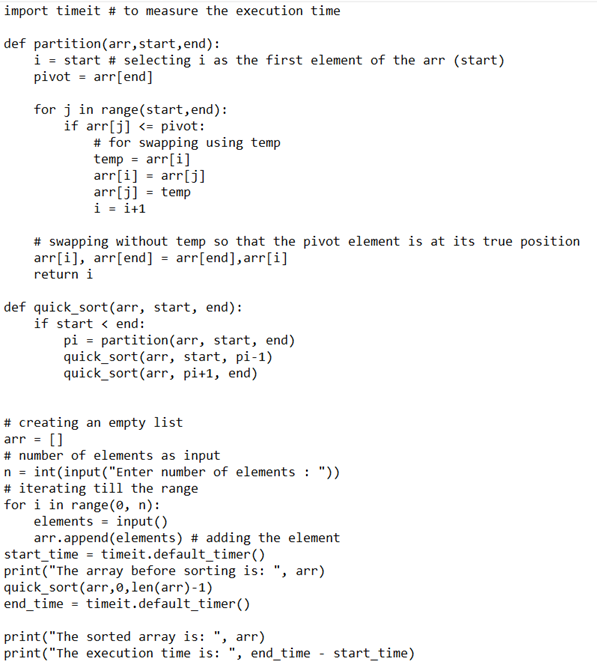
\includegraphics[scale = 0.8]{sourcecode}

5. \textbf{Analysis Results} \\
\indent Time taken by quick sort is: $T(n) = T(k) + T(n-k-1) + \Theta(n)$. The first two terms ($T(k)$ and $T(n-k-1)$) are for two recursive calls, and the last term ($\Theta(n)$) is for the partition process. k is the number of elements that are smaller than a pivot. \\
\indent Let's consider the worst case first. Worst case happened when the first element is the smallest (or say minimum element). In this case, k would be zero then $T(n)$ is: $T(n) = T(0) + T(n-1) + \Theta(n)$, which can be re-written as: $T(n) = T(n-1) + \Theta(n)$, and it's $\frac{cn(n+1)}{2} = O(n^2)$. Thus the solution of above recurrence is $\Theta(n^2)$ \\
\indent Now let's consider the best case. The best case occurs when the partition process always picks the middle element as pivot. It means, $k \approx \frac{k}{2} \approx n-k-1$. Thus $T(n) = T(n/2) + T(n/2) + \Theta(n)$, which is equivalent to $T(n) = 2T(n/2) + \Theta(n)$. And then we can see that the $T(n)$ looks similar to merge sort. We can conclude that $T(n) = O(n\log n)$. It can be also solved using Master Theorem's case 2. \\
I attached each execution result. \\
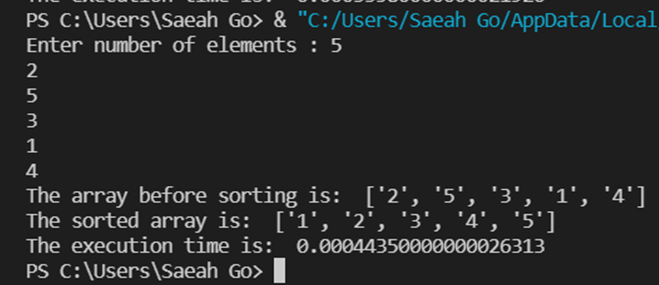
\includegraphics[scale = 0.7]{25314} \\
This is the best case of quicksort, since the 3 is the middle value of the array. We can see that the execution time is about $0.0004435$ seconds.\\
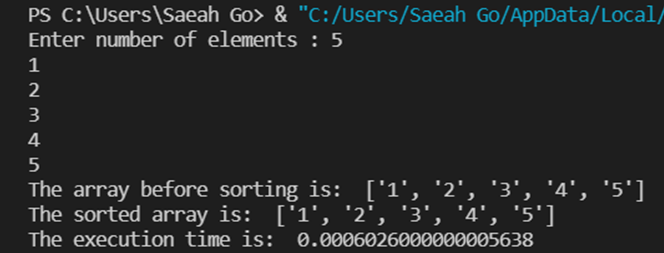
\includegraphics[scale = 0.7]{Ordered 25314} \\
This case is considered as the worst case since it's the ordered array of ``25314". The execution time is about $0.0006026$ seconds, which is bigger than the execution time of ``25314". It satisfies our theoretical assertions.\\
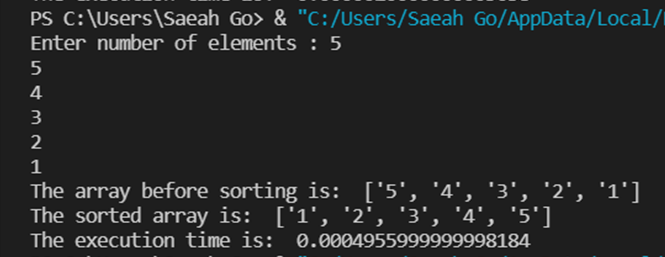
\includegraphics[scale = 0.7]{Reversed 25314} \\
This case is considered as the worst case since the input array is already sorted reversely. The execution time is about $0.0004956$ seconds, which is slightly higher than the execution time of the original array, ``25314".\\
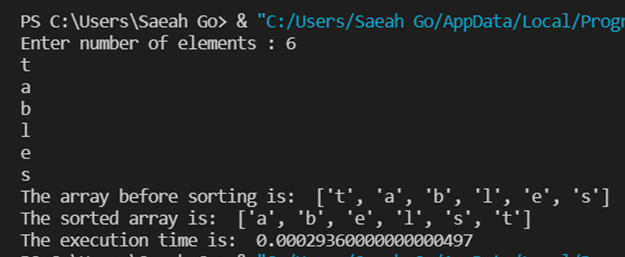
\includegraphics[scale = 0.7]{tables} \\
The array ``tables" is considered as an average case. The execution time is $0.0002936$ seconds. \\
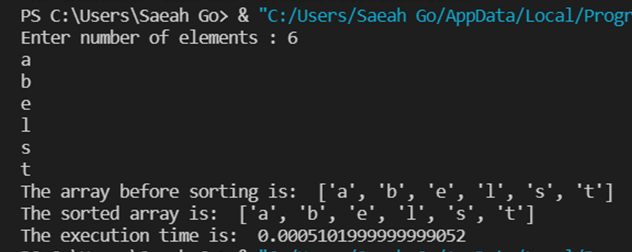
\includegraphics[scale = 0.7]{Ordered tables} \\
The sorted array of tables is ``abelst". In this case, the time execution is about $0.0005102$ seconds which makes sense since the time complexity is $O(n^2)$. \\
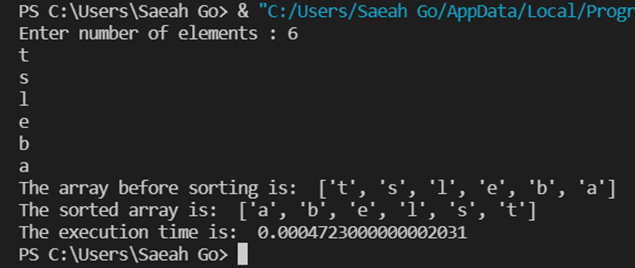
\includegraphics[scale = 0.7]{Reversed tables} \\
The reverse sorted array ``tsleba" has an execution time of $0.0004723$ seconds, which is also bigger than the average case time, $0.0002936$ seconds. \\
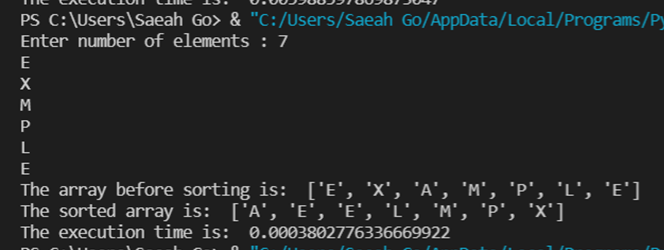
\includegraphics[scale = 0.7]{EXAMPLE} \\
The given array ``EXAMPLE" is considered as an average case, and its execution time is $0.0003803$ seconds. \\
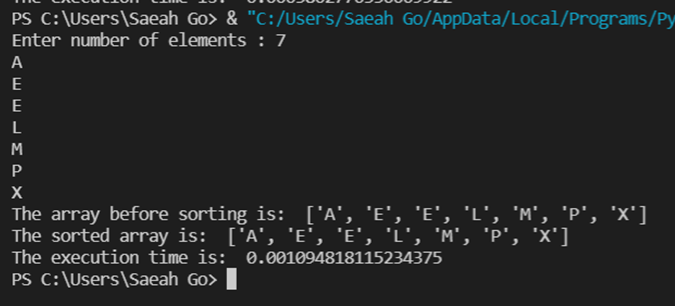
\includegraphics[scale = 0.7]{Ordered EXAMPLE} \\
The ordered array ``AEELMPX" is the worst case, and its execution time is $0.0010948$ seconds, which is much bigger than EXAMPLE's execution time, $0.0003803$ seconds. \\ 
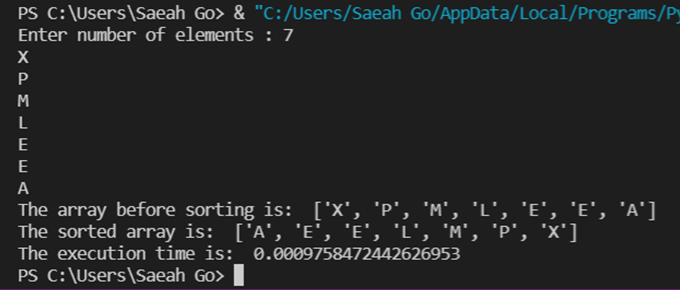
\includegraphics[scale = 0.7]{Reversed EXAMPLE} \\
The reversed array ``XPMLEEA" is also considered as the worst case, its execution time is approximately $0.0009758$ seconds. \\
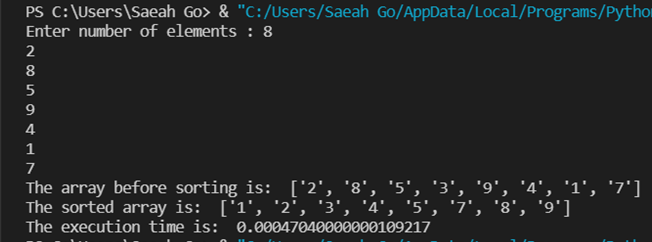
\includegraphics[scale = 0.7]{28539417} \\
The integer array ``28539417" is the average case. Its execution time is $0.0004704$ seconds. \\
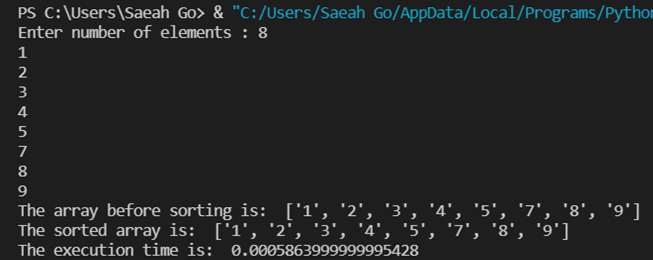
\includegraphics[scale = 0.7]{Ordered28539417} \\
The sorted array of 28539417 is ``12345789". The execution time is approximately $0.0005864$, which is bigger than the average case execution time. \\
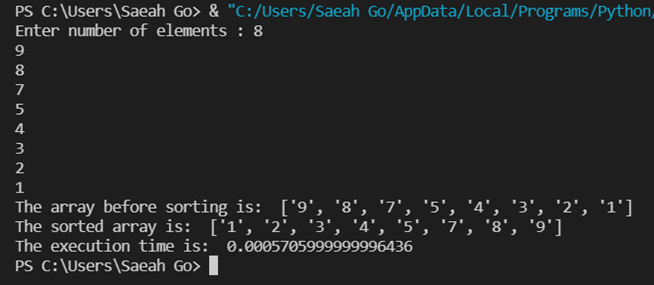
\includegraphics[scale = 0.7]{Reversed 28539417} \\
The reversely sorted array ``98754321"'s execution time is $0.0005706$ seconds, which is close to the sorted array 12345789's execution time and higher than the array 28539417. \\
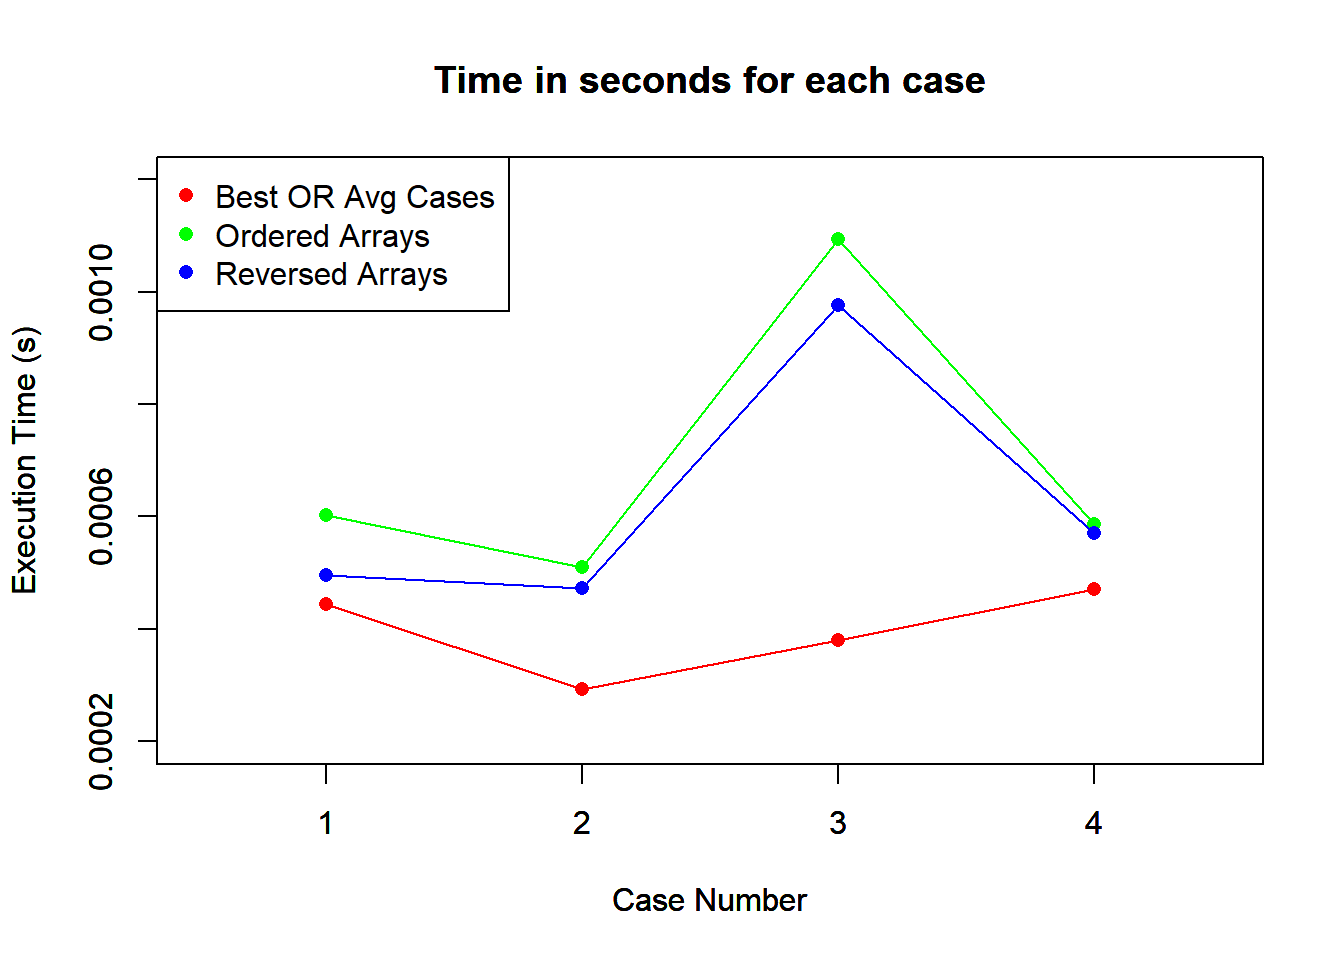
\includegraphics[scale = 0.7]{graph} \\
Through the graph, we could check the fact that in best or average cases (the red dots), it takes less time than the worst cases (ordered arrays, reversed arrays). Also I could find that even though ordered arrays and reversed arrays both are considered as the worst cases, the ordered arrays were more tend to have higher time execution. So I can conclude that when array is sorted, it is the worst case in this quicksort algorithm. \\

6. \textbf{Recommendations} \\ 
It is okay to use the quicksort if you have arrays that the pivot element divides the list into two equal halves by coming exactly in the middle position. When the list is either arranged in ascending or descending order, then the time complexity is $O(n^2)$. So in these cases, it's better to use another sorting algorithm like mergesort, because mergesort has $O(n\log n)$ in all three cases (best, average, and worst cases). Although the worst case time complexity of quicksort is $O(n^2)$ which is more than many other sorting algorithms like merge sort and heap sort, it has the best performance in the average cases for most inputs. So quicksort is generally considered the fastest sorting algorithm. Therefore I recommend using quicksort. \\

7. \textbf{Appendix 1} \\ 
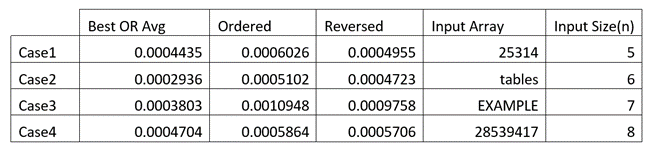
\includegraphics[scale = 0.7]{table} 
This is the table of raw data, which includes input sizes and input arrays exactly what was used in the experiment. \\

8. \textbf{Appendix 2} \\
\indent Case 1 is the integer array. The array is 2, 5, 3, 1, 4. Its input size is 5, and we considered and tested three cases for this. When the array is the average case (2, 5, 3, 1, 4), when the array is sorted (1, 2, 3, 4, 5), and when the array is sorted reversely (5, 4, 3, 2, 1). \\
\indent Case 2 is the character array (specifically lower case) which is t, a, b, l, e, s. The input size is 6, and similarly we did in Case 1, we considered three cases for this array. The average case (t, a, b, l, e, s), the sorted array case (a, b, e, l, s, t), and the reversed sorted array case (t, s, l, e, b, a). \\
\indent Case 3 is also the character array. The given array is E, X, A, M, P, L, E, which consists of all upper cases. Its size is 7, and we tested three cases. The average case (E, X, A, M, P, L, E), the worst cases (A, E, E, L, M, P, X) and (X, P, M, L, E, E, A). \\
\indent Case 4 is the integer array, which is 2, 8, 5, 3, 9, 4, 1, 7. The input size is 8, and we are doing the experiment with three different cases (average case and two worst cases).  
\end{document}
